% filepath: c:\Users\barte\source\repos\mm_projekt\raport.tex
\documentclass[12pt,a4paper]{article}
\usepackage[utf8]{inputenc}
\usepackage{polski}
\usepackage{amsmath}
\usepackage{graphicx}
\usepackage{hyperref}
\usepackage{geometry}
\geometry{margin=2.5cm}

\title{Raport z projektu w ramach przedmiotu \\ Modelowanie Matematyczne}
\author{Bartosz Chabros 198404 \and Beniamin Cymanowski 198067}
\date{\today}

\begin{document}

\maketitle

\section{Cel projektu}
Celem projektu było stworzenie aplikacji umożliwiającej symulację odpowiedzi układu dynamicznego z regulatorem PI na różne typy sygnałów wejściowych. Użytkownik może zmieniać parametry transmitancji, regulatora oraz sygnału wejściowego z poziomu interfejsu graficznego.

\section{Opis układu}
Układ składa się z transmitancji obiektu $G_p(s)$ oraz regulatora PI $G_c(s)$. Całość została zamknięta w pętli sprzężenia zwrotnego.

\subsection{Transmitancja obiektu}
\[
G_p(s) = \frac{a_1 s + a_0}{b_2 s^2 + b_1 s + b_0}
\]

\subsection{Regulator PI}
\[
G_c(s) = K_p + \frac{K_i}{s}
\]

\section{Interfejs użytkownika}
Aplikacja została napisana w języku Python z użyciem bibliotek PyQt6 oraz Matplotlib. Umożliwia ona:
\begin{itemize}
    \item Wprowadzanie parametrów transmitancji i regulatora,
    \item Wybór typu sygnału wejściowego (sinusoidalny, prostokątny, trójkątny),
    \item Ustawienie częstotliwości, fazy, czasu i kroku symulacji,
    \item Wizualizację sygnału wejściowego oraz odpowiedzi układu.
    \item Sprawdza stabilność układu i wyświetla o niej komunikaty w terminalu.
\end{itemize}

\section{Opis działania programu}
Po uruchomieniu programu użytkownik wprowadza parametry, wybiera typ sygnału i uruchamia symulację. Program oblicza odpowiedź układu w dziedzinie czasu, korzystając z modelu stanu oraz wybranego sygnału wejściowego.

\section{Przykładowe wyniki}
\begin{figure}[h!]
    \centering
    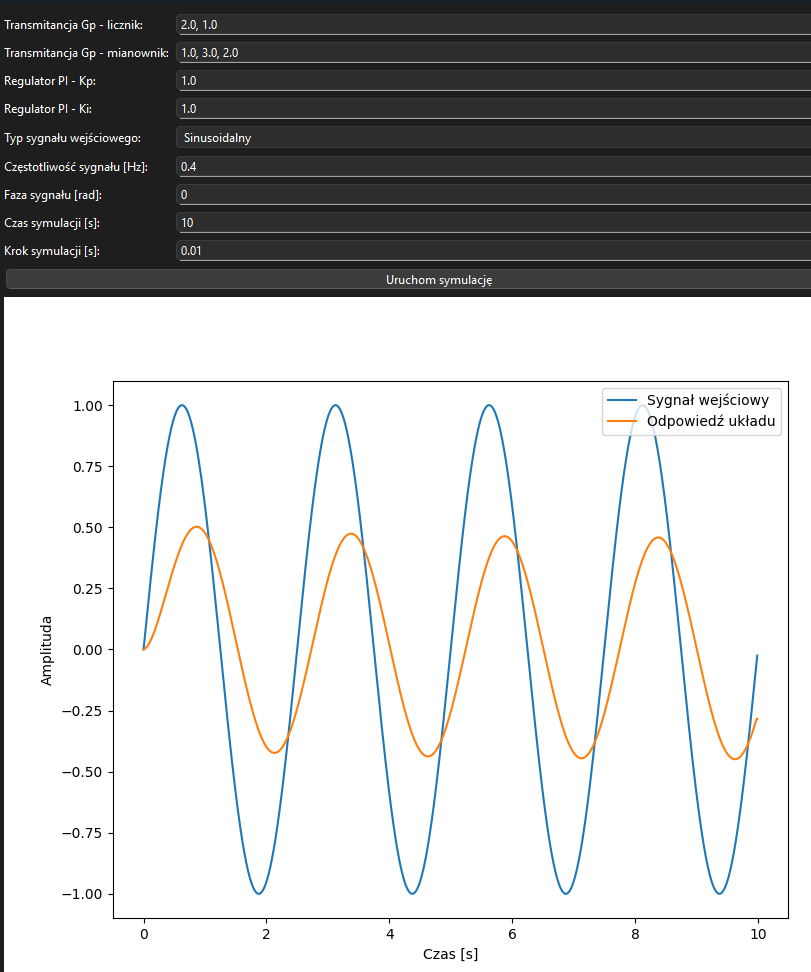
\includegraphics[width=0.8\textwidth]{wykres1.png}
    \caption{Przykładowa odpowiedź układu na sygnał sinusoidalny.}
\end{figure}



\section{Wnioski}
Projekt pozwolił na praktyczne zastosowanie wiedzy z zakresu teorii sterowania oraz programowania. Aplikacja umożliwia szybkie testowanie wpływu parametrów na odpowiedź układu.



\end{document}